\section{Desarrollo}
\subsection{Desv\'ios}

En este experimento realizamos un an\'alisis sobre los desv\'ios de los vuelos en base al tiempo. Dividimos al año en 12 meses y tomamos el per\'iodo 2000-2008. Para generar un an\'alisis representativo del comportamiento a escala pa\'is decidimos tomar 2 estados con caracter\'isticas particulares: deben tener gran cantidad de vuelos de llegada y deb\'ia ser uno de cada costa. De este modo tomamos a los estados de California y Florida para realizar el an\'alisis.

\subsubsection{California}

En el siguiente gr\'afico se puede observar el porcentaje de vuelos desviados en el per\'iodo mencionado para vuelos con destino a California.

\begin{figure}[h!]
  \begin{center}
	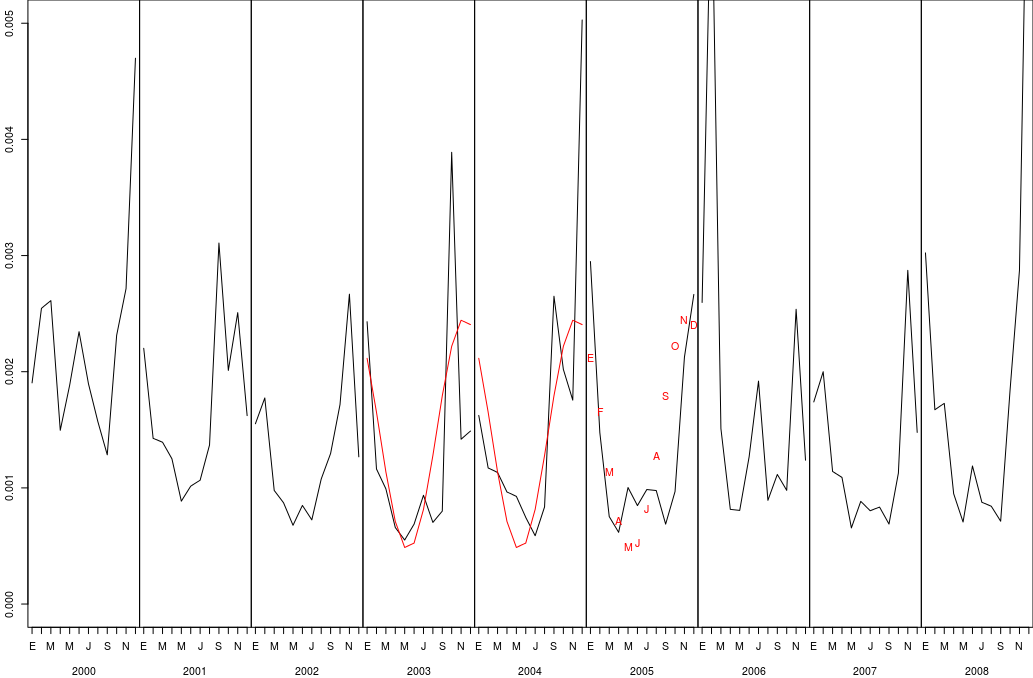
\includegraphics[scale=0.4]{img/plot_CA_2003-2005.png}
	\caption{Diverted arrivals - California}
  \end{center}
\end{figure}

Para aproximar a la funci\'on observamos algunas cosas:
\begin{itemize}  
\item Hay cierta periodicidad en la funci\'on. Posee picos en los meses correspondientes a las vacaciones de verano del hemisferio norte y descensos en el resto. El per\'iodo es de 12 meses.
\item Aunque la funci\'on tiene picos marcados, su forma se asemeja a la de $sin$ y $cos$.
\end{itemize}

Dados estos indicios nos proponemos encontrar una familia de funciones para aproximar nuestro gr\'afico usando cuadrados m\'inimos. Estas funciones ser\'an una combinaci\'on de $sin$ y $cos$ con per\'iodo 12. Las siguientes 2 familias de funciones responden a estas caracter\'isticas y aproximan relativamente bien a nuestra funci\'on, dados $alpha_i$ correspondientes.


$F_1 = \alpha_1 * abs(sin(\frac{\pi}{12}*x) * cos(\frac{\pi}{6}*x)^2) + \alpha_2$

$F_2 = \alpha_1 * sin(\frac{\pi}{6}*x) + \alpha_2 * cos(\frac{\pi}{6}*x) + \alpha_3$


La primera multiplica al $sin$ y $cos$ y toma el valor absoluto para eliminar los picos negativos. La segunda realiza la suma de los $sin$ y $cos$. No es relevante ac\'a tomar el valor absoluto ya que no hay picos marcados negativos. Luego a ambas funciones le sumamos una constante para que la curva se desplace en direcci\'on vertical. Observamos que sumar una variable lineal no ten\'ia impacto apreciable en la aproximaci\'on. 

Luego resolvimos cuadrados m\'inimos para ambas funciones y calculamos el error cuadr\'atico medio de cada una. Como training tomamos a los años 2003 y 2004 e intentamos predecir 2005.

Los errores cuadr\'aticos medios son: $ECM(F_1) = 0.0003236866$ y $ECM(F_2) = 0.0002451076$, siendo la segunda funci\'on una mejor aproximaci\'on que la primera. Los valores son pequeños ya que las mediciones son sobre un porcentaje pequeño.

Por lo tanto se puede ver en el gr\'afico anterior la aproximaci\'on que $F_2$ realiza en la muestra, prediciendo c\'omo ser\'a 2005. Se ve que respeta el comportamiento general y aproxima el pico que hay a principio y fin de año.

\subsubsection{Florida}

Realizamos el mismo an\'alisis para los vuelos dirigidos a Florida. Tomamos los mismos 
La funci\'on sigue teniendo un comportamiento peri\'odico año a año, pero en este caso vemos que por alg\'un motivo hay un desplazamiento horizontal de la curva: los picos positivos se encuentran a mitad de año.
Por otro lado, el porcentaje de vuelos desviados est\'a en el mismo rango que en California.
Dado este conjunto de similitudes y diferencias con el caso anterior, nos interes\'o ver c\'omo se comportaban nuestras familias de funciones anteriores para aproximar a nuestra nueva curva.

Para esto realizamos cuadrados m\'inimos con las siguientes dos familias de funciones:

$F_1 = \alpha_1 * abs(sin(\frac{\pi}{12}*x) * cos(\frac{\pi}{6}*x)^2) + \alpha_2$

$F_2 = \alpha_1 * sin(\frac{\pi}{6}*x) + \alpha_2 * cos(\frac{\pi}{6}*x) + \alpha_3$

y vimos que los errores cuadr\'aticos medios en este caso fueron de $ECM(F_1) = 0.0003098236$ y $ECM(F_2) = 0.0003590168$, o sea, bastante similares al anterior.

Se puede observar la curva en el siguiente gr\'afico:

\begin{figure}[h!]
  \begin{center}
	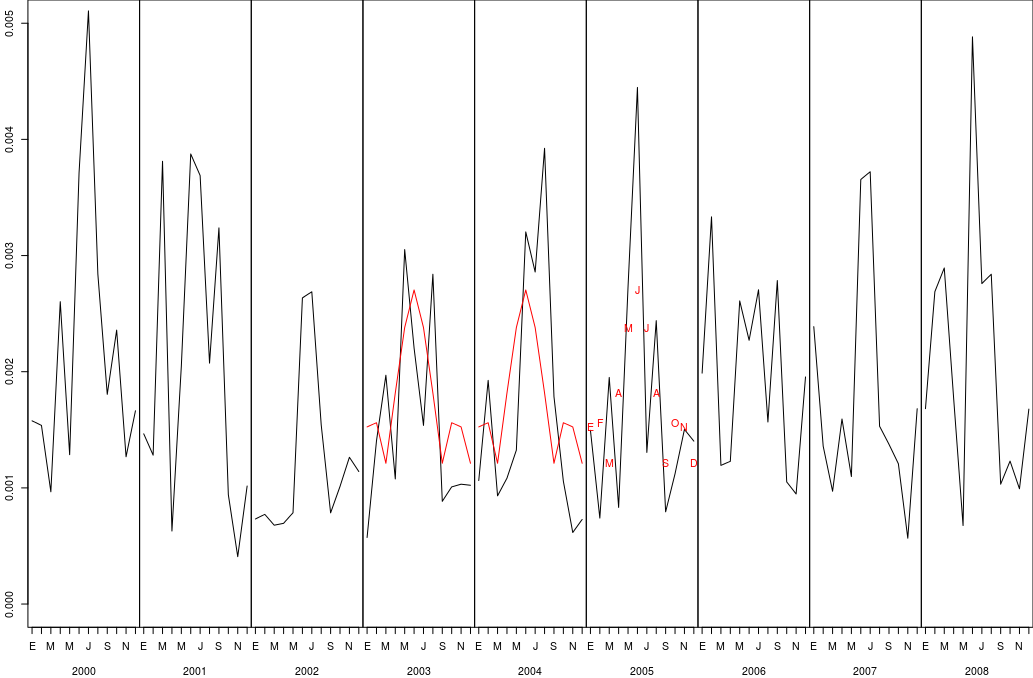
\includegraphics[scale=0.4]{img/plot_FL_2003-2005.png}
	\caption{Diverted arrivals - Florida}
  \end{center}
\end{figure}

Pero como se ve, los picos del medio son muy pronunciados, entonces quisimos crear una familia de funciones parecida  a las que ten\'iamos pero que considerase esa particularidad.
Probando un poco nos dimos cuenta que las potencias de $cos$ tienen un comportamiento de este estilo. Por ejemplo $5*cos(x)^{500} + 1$ tiene el siguiente gr\'afico:

\begin{figure}[h!]
  \begin{center}
	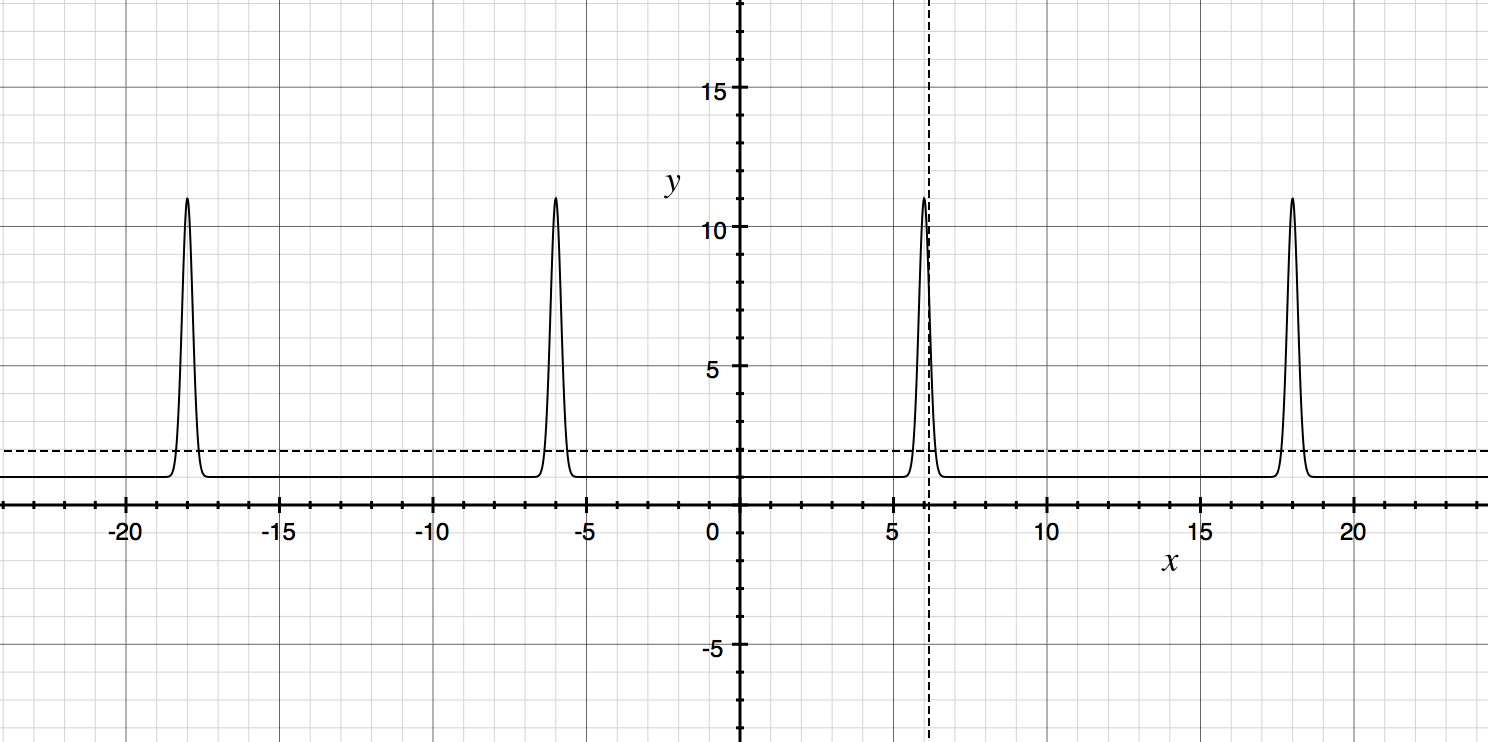
\includegraphics[scale=0.4]{img/cos500.png}
	\caption{$5*cos(x)^{500} + 1$}
  \end{center}
\end{figure}

Por lo tanto llegamos a la siguiente familia de funciones que usa esta nueva t\'ecnica.

$F_3 = \alpha_1 * abs(sin(\frac{\pi}{12}*x) * cos(\frac{\pi}{6}*x)^2) + \alpha_2 * cos(\frac{\pi}{12}*x - \frac{\pi}{2})^{500} + \alpha_3$

El error cuadr\'atico medio de esta funci\'on es $ECM(F_3) = 0.00030524$.

Podemos ver a $F_3$ representada en el gr\'afico de Florida en rojo. En ese caso se entren\'o cuadrados m\'inimos con 2003 y 2004 y se predice 2005.








